\section{Introduction}
\label{sec_introduction}

Human speech is captured by microphones constantly. Dialogues or utterances are recorded at online meetings, for creating content, and for being aided by virtual assistants or service providers. Many of these recordings inevitably require automated processing, for which the common approach is to run automatic speech recognition (ASR) systems that convert audio to transcribed text. The produced transcript is then handled
%more efficiently by humans or 
with spoken language understanding (SLU) technology. 

Considerable effort is invested in developing ASR systems that can overcome environmental sounds, vague speech and phenomena of spoken language,
%often present in audio files, 
in order to produce transcripts that are as faithful to the speech (``clean'') as possible \citep{iwamoto2022artifacts, Prabhavalkar2023surveyASR}. In turn, the text processing step can be performed more effectively. Simply put, the mistakes (``noise'') produced in the speech-to-text stage propagate to downstream tasks in the text processing stage \citep{kubis-etal-2023-back, feng2022asrglue}.

% !TEX root = main.tex

\begin{figure}[t]
\vspace{-1.5cm}
\begin{minipage}{0.34\textwidth}
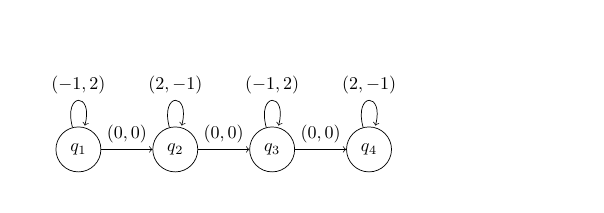
\begin{tikzpicture}[scale=0.25]
\usetikzlibrary{automata, positioning}
\scalebox{0.65}{
\node[state] (q1) {$q_1$};
\node[state, right=of q1] (q2) {$q_2$};
\node[state, right=of q2] (q3) {$q_3$};
\node[state, right=of q3] (q4) {$q_4$};

\path[->] (q1) edge [loop above] node[above] {$(-1,2)$} (q1) edge node[above] {$(0,0)$} (q2); 
\path[->] (q2) edge [loop above] node[above] {$(2,-1)$} (q2) edge node[above] {$(0,0)$} (q3);
\path[->] (q3) edge [loop above] node[above] {$(-1,2)$} (q3) edge node[above] {$(0,0)$} (q4);
\path[->] (q4) edge [loop above] node[above] {$(2,-1)$} (q4);
}
\end{tikzpicture}
\end{minipage}
\begin{minipage}{0.32\textwidth}
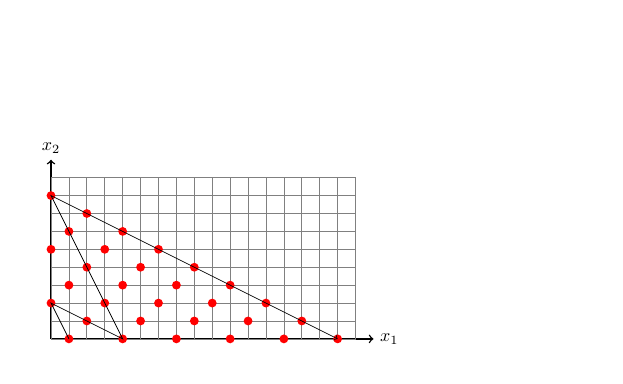
\begin{tikzpicture}[scale=0.35]
\scalebox{0.65}{
\draw[->, thick] (0, 0) -- (18, 0) node[right] {$x_1$};
\draw[->, thick] (0, 0) -- (0, 10) node[above] {$x_2$};

\draw[step=1, gray, thin] (0, 0) grid (17, 9);

\foreach \x in {1,4,7,10,13,16} \fill[red] (\x,0) circle (7pt);
\foreach \x in {2,5,8,11,14} \fill[red] (\x,1) circle (7pt);
\foreach \x in {0,3,6,9,12} \fill[red] (\x,2) circle (7pt);
\foreach \x in {1,4,7,10} \fill[red] (\x,3) circle (7pt);
\foreach \x in {2,5,8} \fill[red] (\x,4) circle (7pt);
\foreach \x in {0,3,6} \fill[red] (\x,5) circle (7pt);
\foreach \x in {1,4} \fill[red] (\x,6) circle (7pt);
\foreach \x in {2} \fill[red] (\x,7) circle (7pt);
\foreach \x in {0} \fill[red] (\x,8) circle (7pt);

\draw[->] (1,0) -- (0,2) -- (2,1) -- (4,0) -- (3,2) -- (2,4) -- (1,6) -- (0,8) -- (2,7) -- (4,6) -- (6,5) -- (8,4) -- (10,3) -- (12,2) -- (14,1) -- (16,0);
}
\end{tikzpicture}
\end{minipage}
\begin{minipage}{0.32\textwidth}
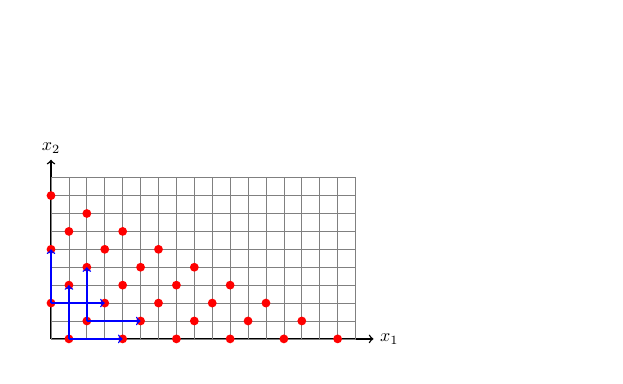
\begin{tikzpicture}[scale=0.35]
\scalebox{0.65}{
\draw[->, thick] (0, 0) -- (18, 0) node[right] {$x_1$};
\draw[->, thick] (0, 0) -- (0, 10) node[above] {$x_2$};

\draw[step=1, gray, thin] (0, 0) grid (17, 9);

\foreach \x in {1,4,7,10,13,16} \fill[red] (\x,0) circle (7pt);
\foreach \x in {2,5,8,11,14} \fill[red] (\x,1) circle (7pt);
\foreach \x in {0,3,6,9,12} \fill[red] (\x,2) circle (7pt);
\foreach \x in {1,4,7,10} \fill[red] (\x,3) circle (7pt);
\foreach \x in {2,5,8} \fill[red] (\x,4) circle (7pt);
\foreach \x in {0,3,6} \fill[red] (\x,5) circle (7pt);
\foreach \x in {1,4} \fill[red] (\x,6) circle (7pt);
\foreach \x in {2} \fill[red] (\x,7) circle (7pt);
\foreach \x in {0} \fill[red] (\x,8) circle (7pt);

\draw[->,blue,thick] (1,0) -- (4,0);
\draw[->,blue,thick] (1,0) -- (1,3);

\draw[->,blue,thick] (2,1) -- (5,1);
\draw[->,blue,thick] (2,1) -- (2,4);

\draw[->,blue,thick] (0,2) -- (3,2);
\draw[->,blue,thick] (0,2) -- (0,5);
}
\end{tikzpicture}
\end{minipage}
\caption{Left: 4-component \dvass $V_2$. 
Middle: the set $\reach_{q_4}(V_2, q_1(1,0))$ and a path $q_1(1,0) \tran q_4(16,0)$.
Right: bases 
%$A = \{(1,0),(2,1),(0,2)\}$ 
and periods 
%$P = \{(0,3),(3,0)\}$
 of an over-approximating semi-linear set $A+P^*$.}
\label{fig:zigzag}
\end{figure}

\begin{example}
For $k\geq 1$, let $V_k$ be a $(2k)$-component \dvass, where each component has just one state $q_i$
and one transition:
$(q_i, (-1,2), q_i)$ for odd $i$, and $(q_i, (2,-1), q_i)$ for even $i$.
Bridge transitions are $(q_i, (0,0), q_{i+1})$.
Figure~\ref{fig:zigzag} shows $V_2$ (left) and 
a path in $V_2$ from $s = q_1(1,0)$ to $t = q_4(16,0)$ together with 
the reachability set $\reach_{q_4}(V_2, s)$ (middle).
In general,
\begin{align} \label{eq:reachk}
X_k := \reach_{q_{2k}}(V_k, s) \ = \ \set{(x_1,x_2) \mid x_1+2x_2 \leq 4^k, \  x_1+2x_2 \equiv 1 \!\! \mod 3}.
\end{align}
Even if the size of the reachability set is 
exponential in $k$, for small $(x_1, x_2)$ it is periodic and the periods are small.
The set $X_k$ can be over-approximated by $A + P^*$ for $A = \set{(1,0),(2,1),(0,2)}$ and $P = \set{(0,3),(3,0)}$
(shown on the right of Figure~\ref{fig:zigzag}), namely for every $k\geq 1$ and $B\in\N$,
the set $X_k$ is \kanapka {$8$} {$B$}. 
For illustration, consider $Y := X_k \cap ((1,0) + P^*)$.
If $(1,0) + P^{\leq B} \subseteq X_k$ then $Y$ is a $B$-approximation
of $(1,0) + P^*$ with $\norm((1,0)), \norm(P) \leq 3 \leq 8$. 
Otherwise, there is some $(v_1, v_2) \in \big((1,0) + P^{\leq B}\big)\setminus X_k$, and
then $B$ is larger than $4^k$:
\[
%8B \geq 2(1 + 3B) \geq 2(v_1 + v_2) \geq v_1 + 2 v_2 > 
4^k < v_1 + 2 v_2 \leq 2(v_1 + v_2) \leq 2(1+3B) \leq 8B.
\]
Therefore by \eqref{eq:reachk}, each $(x_1,x_2) \in Y$ satisfies 
$\norm(x_1,x_2) = x_1 + x_2 \leq x_1 + 2x_2 \leq 4^k < 8B$, and thus
$Y$, seen as a union of singletons, is a union of 
linear sets with norm of base bounded by $8B$ and empty set of periods. 
In both cases, 
$Y$ is \kanapka {$8$} {$B$}. 
%The same intuition stays behind polynomial approximability of \dvass stated in Lemma~\ref{lem:2vass-sandwich}.
\end{example}

Eventual SLU tasks are abundant, from traditional dialog act classification \citep{shriberg-etal-2004-icsi} to summarization \citep{Waibel1998summ} and even neurological assessment of speakers \citep{Roshanzamir2021Alzheimer}. 
Indeed, over the years studies have noticed that noisy transcripts burden NLP models, and actions are consequently taken to work around or mitigate the noise (surveyed in Section \ref{sec_related_work}). Furthermore, different downstream tasks are not alike in how they respond to the amount and types of errors in transcripts. Some are highly vulnerable to errors, while others may tolerate more noise, or specific types of noise, depending on a task's requirements (as demonstrated in our analyses in Section \ref{sec_results}).
\autoref{fig_example} shows an utterance transcribed with varying levels of error severity, causing unpredictable behavior in downstream understanding tasks. 
Importantly, the standard word error rate (WER) metric, that measures the amount of errors in generated transcripts, does not capture discrepancies in types of noise, and cannot forecast results on downstream tasks \citep{wang2003indicator}.
%\ac{I would add that WER does not capture this, so we suggest a new method that does capture it}.

%Moreover, SLU pipelines have interchangeable components tasks, such as the ASR and NLP task models, that influence the downstream task differently.
%\ac{I think the following paragraph somewhat diminishes our contribution, consider move most of it to related work}
%Indeed, over the years there have been many studies that assess the influence of ASR noise on downstream tasks, as well as proposed methods for cleaning transcripts to reduce propagating errors (detailed in Section \ref{sec_related_work}). These studies have been conducted based on varying ASR models, in various speech domains, and with inconsistent evaluation techniques. Interestingly, each study draws somewhat different conclusions, but all have something in common: they strive to determine whether ASR-produced transcripts are sufficiently reliable for completing their particular task.

Drawing upon lessons from previous research on SLU, in this work we propose a 
%general-purpose
framework for systematically analyzing the \textit{\textbf{e}}ffect of transcription \textit{\textbf{n}}oise on a \textit{\textbf{dow}}nstream task (\ENDow; Section \ref{sec_framework}). Our first-of-its-kind framework examines task model behavior under varying noise intensities and types, providing quantitative metrics and facilitating qualitative analyses.
It determines acceptable noise levels for a downstream task, identifies effective transcript-cleaning techniques, and supports planning and implementation of SLU solutions.
Previous studies have examined aspects of \ENDow{}, but always within the scope of a specific task or use case. We suggest that, especially in the era of generalized models and benchmarks, there is a need for a versatile framework that consistently analyzes and compares SLU solutions.
%It provides quantitative scores and enables qualitative analysis, to conveniently compare and contrast competing SLU pipelines.
The components in the framework's pipeline, such as the ASR system or task model, are flexibly configured to perform controlled examinations.
%for SLU pipeline comparisons.
%The framework helps practitioners determine acceptable noise levels for a downstream task and identify effective transcript-cleaning techniques.
% it allows practitioners
% %-- academic or industrial -- 
% to inspect how much noise is acceptable for an intended downstream task, and which transcript-cleaning techniques can effectively aid the task model. 
%Such a methodical procedure allows the practitioner to establish a speech-to-downstream-task pipeline that is adequate for their specific use-case.

%\ac{Before diving into the details, give a sentence about the novelty and goal of the framework} 

Given an SLU dataset, the framework prepares audio files, with varying levels of acoustic distortion, which are then transcribed by an ASR system, producing transcript sets with increasing levels of transcription noise. A method of transcript cleaning then adjusts noise \textit{types}, generating additional transcript versions. Finally, a downstream task model is applied, allowing comparison and analysis across the transcript versions.
Notably, beyond its configurable pipeline, the framework supports any task dataset, including non-spoken language datasets, greatly expanding the scope for assessing \ENDow{}.
%Given an SLU dataset, the framework prepares audio files with varying levels of acoustic distortion, after which an ASR system transcribes the audio. This results in several versions of transcript sets, each with an increasing level of transcription noise. Transcripts are then repaired with a cleaning method of choice that adjusts the \textit{types} of noise, producing additional versions of transcript sets. The model of a downstream task is then applied on the various versions of transcripts, yielding task results that can be compared and analyzed across versions.
% Given an SLU dataset, the framework systematically degrades the input audio files at varying intensities, 
% simulating different acoustic conditions,
% after which an ASR system transcribes the audio. This results in several versions of transcript sets, each with an increasing level of transcription noise. Transcripts are then repaired with a cleaning method of choice that adjusts the \textit{types} of noise, producing additional versions of transcript sets. The model of a downstream task is then applied on the various versions of transcripts, yielding task results that can be compared and analyzed across versions.

%Given a set of audio recordings, the framework adds background noise and reverberation at different levels to the recordings. All audio files are then transcribed with an ASR system, and the transcripts are cleaned post-hoc with a cleaning method of choice. Next, the sets of transcripts are passed to the model that conducts the downstream task, and all the results can subsequently be compared at different noise levels and cleaning approaches. The resulting analysis informs what noise level is acceptable for the downstream task, and which cleaning methods efficiently contribute to the end results.

We exemplify the use of our framework (Section \ref{sec_setup}), and perform an extensive analysis (Section \ref{sec_results}) across three SLU tasks, with seven intensities of noise, seven cleaning techniques, and four LLM task models. Specifically, we focus on %meeting
summarization
%as a generation task 
\citep{zhong-etal-2021-qmsum}, %transcript
question-answering
%as an extraction task 
\citep{wu-etal-2022-qaconv}, and dialog-act classification
%categorization as a classification task 
\citep{shriberg-etal-2004-icsi}, all from existing SLU datasets. 
%We use Whisper \citep{Radford2023whisper} as the ASR system, and clean transcripts according to part-of-speech types and named entities. To carry out the downstream tasks, we use Llama \citep{grattafiori2024llama3herdmodels}, Mistral \citep{jiang2023mistral7b} and GPT \citep{openai2024gpt4ocard} family models in zero-shot mode.
%\ac{I would add that experimenting with different noise level allow us to isolate phenomena that are overwise are hard to spot (for example, things that we see in high noise scenario are hard to discern in low noise setups}

The results of our diversified experiments yield many insights regarding the level of noise that is acceptable for the downstream tasks, and the impact of the \textit{type} of errors in the transcripts. For example, we observe that named entities are usually the most important term-types for dealing with the tasks, while, surprisingly, verbs are seemingly not as essential. Some findings are unique to specific tasks and models, while others are more consistent. For instance, it is apparent in our experiments that there is a certain amount of noise from which it is not worth the trouble of reducing it. However, that intensity fluctuates with respect to the task, the model, and the type of noise.
The framework also reveals phenomena that occur at particular noise levels, as well as gradual changes as noise increases. For example, we find that GPT-4o-mini \citep{openai2024gpt4ocard} outperforms other models on summarization when transcript noise is low, but the other models overtake GPT as noise increases.
Such findings are valuable for identifying commonalities and differences among various SLU configurations, helping to prioritize efforts for achieving satisfactory outcomes on a downstream task.

% The rest of the paper is structured as follows. Section \ref{sec_related_work} provides background and surveys related works that address the issue of transcript noise in downstream tasks. In Section \ref{sec_framework}, we describe the framework for assessing \ENDow{}. Section \ref{sec_setup} explains the experimental setup for which we exemplify our framework. Finally, Section \ref{sec_results} discusses the results and insights of our experiments.







%The results of our diversified experiments yield several insights regarding the level of noise that is acceptable for the downstream tasks, and the impact of the \textit{type} of errors in the transcripts, across tasks and models. For example, the summarization and question-answering results seem to be only marginally effected when input transcripts contain up to an average word-error-rate of approximately 0.2 (i.e., when $\sim$20\% of words were transcribed erroneously). However the rate changes substantially from one model to another. Moreover, some task models are comparably more effective at lower noise levels, while others are more at higher noise levels. From the repaired transcripts, we generally observe that named entities are usually the most important word types for dealing with the tasks, while, surprisingly, verbs are seemingly not as essential. In this matter, too, the extent of the behavior slightly varies across models. Such findings are desirable for examining the commonalities and differences of varying SLU configurations, emphasizing where to focus efforts in order to attain satisfactory results.

%However, GPT seems to be more robust... named entities important... \todo{Write some findings here}.
%Also, we found that the cleaning approach we use causes a degradation in grammaticality, which, with the models used, seems to be tolerable on transcript-level tasks, but less so on the utterance-level task of dialog-act classification. Such insights are important when designing solutions for transcript-based SLU tasks.

